\documentclass[10pt]{article}

\usepackage[T1]{fontenc}
\usepackage[utf8]{inputenc}
\usepackage{lmodern}
\usepackage[margin=1in]{geometry}
\usepackage{microtype}
\usepackage{booktabs}
\usepackage{array}
\usepackage{enumitem}
\usepackage{xspace}
\usepackage{xcolor}
\usepackage{tikz}
\usetikzlibrary{arrows.meta,positioning,fit,shapes.geometric}
\usepackage[numbers,sort&compress]{natbib}
\usepackage{hyperref}

\definecolor{builderblue}{HTML}{2563EB}
\definecolor{testergreen}{HTML}{15803D}
\definecolor{attackred}{HTML}{B91C1C}
\definecolor{gategray}{HTML}{475569}
\hypersetup{
  colorlinks=true,
  linkcolor=builderblue,
  citecolor=testergreen,
  urlcolor=builderblue,
  pdftitle={Evidence-Driven Generative Development},
  pdfauthor={Ya-Lun Li}
}

\newcommand{\method}{\textsc{EDGD}\xspace}
\newcommand{\mskill}{\textsc{MSkill}\xspace}
\newcommand{\testspec}{\textsc{TestSpec}\xspace}

\title{Evidence-Driven Generative Development:\\
Closed-Loop Synthesis with Independent Testing and Adversarial Differential Gates}
\author{Ya-Lun Li\\Independent Researcher\\\href{mailto:allen7575@gmail.com}{allen7575@gmail.com}}
\date{August 2026}

\begin{document}
\maketitle

\begin{abstract}
Large language models can generate useful software from natural-language requests, but a generated implementation is neither a durable specification nor trustworthy evidence of its own correctness. We present \emph{evidence-driven generative development} (\method), a specification-first workflow in which human-readable behavioral contracts, executable demonstrations, constrained test specifications, and replayable browser evidence are durable artifacts while generated code remains disposable. The workflow separates three model roles. A Builder synthesizes an implementation and public tests; an independent Tester first reviews the untrusted contract and then writes tests in a non-executable domain-specific language; and a bounded Attacker inserts a trusted, known-reject canary into a poisoned copy of an otherwise acceptable contract. A differential gate permits generation only when a fresh Tester allows the original and a second fresh Tester rejects the poisoned variant. Candidate repair then proceeds through public and hidden tests, sandboxed execution, installation, real-environment interaction, and screenshot-backed visual checks. Failures are classified before being promoted into shared policy or skill-specific constraints. We describe the architecture, threat model, acceptance matrix, criterion-evolution rules, and a browser-extension case study. This paper is a methods and systems report: it defines falsifiable evaluation protocols and reports engineering observations, but does not claim that model-based review or finite testing proves semantic safety.
\end{abstract}

\section{Introduction}

Code-generating language models make repeated sampling a practical way to obtain working programs, but functional success varies across samples and tasks \citep{chen2021codex}. Treating one generated program as the permanent source of truth therefore discards a central advantage of generative systems: an implementation can be replaced when the underlying intent remains stable. At the same time, replacing hand-written code with prose alone creates two hazards. First, prose is incomplete until exercised against observable behavior. Second, prose supplied to an agent may contain adversarial instructions, including indirect prompt injection that blurs the boundary between data and instructions \citep{greshake2023indirect,yi2023bipia}.

We ask: \emph{What should remain durable if executable code is regenerated, and what evidence is sufficient to install a generated implementation?} Our answer is \method, a workflow organized around four principles:

\begin{enumerate}[leftmargin=*,itemsep=2pt]
  \item preserve a human-readable contract and a minimal real-world demonstration, not a particular generated implementation;
  \item separate generation, independent specification, and adversarial mutation into isolated roles;
  \item enforce tests through a bounded, non-executable DSL and a trusted Runner rather than trusting model explanations; and
  \item evolve criteria from reproducible failures while retaining implementation freedom wherever evidence does not require a mechanism.
\end{enumerate}

The process resembles counterexample-guided inductive synthesis (CEGIS), in which candidate programs are iteratively refined using verifier-produced counterexamples \citep{solarlezama2006sketching}. It differs in three important respects: its specification begins as a human-readable product contract; its oracle is deliberately plural, combining constrained tests, runtime policy, real-browser interaction, and visual evidence; and its security gate challenges the interpretation of the specification before candidate generation.

This paper contributes:

\begin{itemize}[leftmargin=*]
  \item a durable-artifact model for LLM-generated software;
  \item a three-role closed loop with an explicit differential security matrix;
  \item a trusted, template-driven attacker that tests prompt-injection resistance without granting another model freedom to author arbitrary malicious instructions;
  \item a rule for separating global framework failures, skill-specific contract failures, and disposable candidate defects; and
  \item a reproducible evaluation protocol spanning declarative tests, sandbox policy, installation, real interactions, and screenshots.
\end{itemize}

\section{Background and Motivation}

Property-based testing showed the value of expressing general properties and generating diverse inputs rather than relying only on hand-picked examples \citep{claessen2000quickcheck}. Differential testing compares independent implementations or executions to expose inconsistencies \citep{mckeeman1998differential}. LLM-based red teaming extends automated test generation to behaviors that are difficult to enumerate manually \citep{perez2022redteaming,ganguli2022redteaming}. Interactive benchmarks further show that success in a static benchmark does not imply reliable operation in a real graphical environment \citep{xie2024osworld}.

\method combines ideas from these traditions but addresses a different unit of development. The unit is a small, installable capability described by a readable contract. In our reference system, MonkeySkill, such a contract is called an \mskill{} \citep{monkeyskill2026}. The contract declares modes, capabilities, denied effects, compatibility requirements, and observable criteria. A language model generates JavaScript and CSS only after the security gate has accepted the contract.

The central design tension is that a strict implementation recipe improves repeatability but destroys generative freedom, while an unconstrained prompt preserves freedom but weakens reproducibility. \method resolves this tension with three layers:

\begin{enumerate}[leftmargin=*]
  \item \textbf{Behavioral contract:} required observable outcomes and forbidden effects; strict and durable.
  \item \textbf{Validated implementation constraints:} mechanisms or ordering constraints retained only after repeated evidence shows they are necessary for this specific capability.
  \item \textbf{Free implementation detail:} algorithms, data structures, naming, and organization remain Builder choices.
\end{enumerate}

\section{Durable Artifacts}

Generated source is treated as a derivative. The durable record consists of:

\begin{description}[leftmargin=2.7cm,style=nextline]
  \item[Demo] A minimal reproduction of the motivating failure, with a visible blocked baseline and expected restored behavior.
  \item[Contract] A human-readable \mskill{} plus a declarative manifest of capabilities and denied effects.
  \item[Criteria] Stable, uniquely identified behavioral outcomes justified by evidence.
  \item[Test DSL] Builder-authored public and Tester-authored independent \testspec{} documents using the same bounded grammar.
  \item[Runner] A trusted interpreter that constructs fixtures, applies actions, observes allowed state, and enforces capability policy.
  \item[Evidence] Candidate hashes, test outcomes, browser observations, screenshots, and preserved failure reproductions.
\end{description}

This split allows multiple implementations to satisfy one contract while keeping validation replayable. It also makes a safety boundary explicit: a behavior that the DSL and Runner cannot enforce is \emph{unverifiable}, not silently safe.

\section{Closed-Loop Architecture}

Figure~\ref{fig:pipeline} shows the mainline. Tester A reviews the original contract as untrusted data. Only an \texttt{allow} verdict advances to the Attacker. The trusted orchestrator uses the Attacker's allowlisted plan to construct a poisoned variant. Fresh Tester B sees only that variant and is not told the expected answer. Only the pair \texttt{allow}/\texttt{reject} releases the original contract---never the poisoned copy---to Builder.

\begin{figure*}[t]
\centering
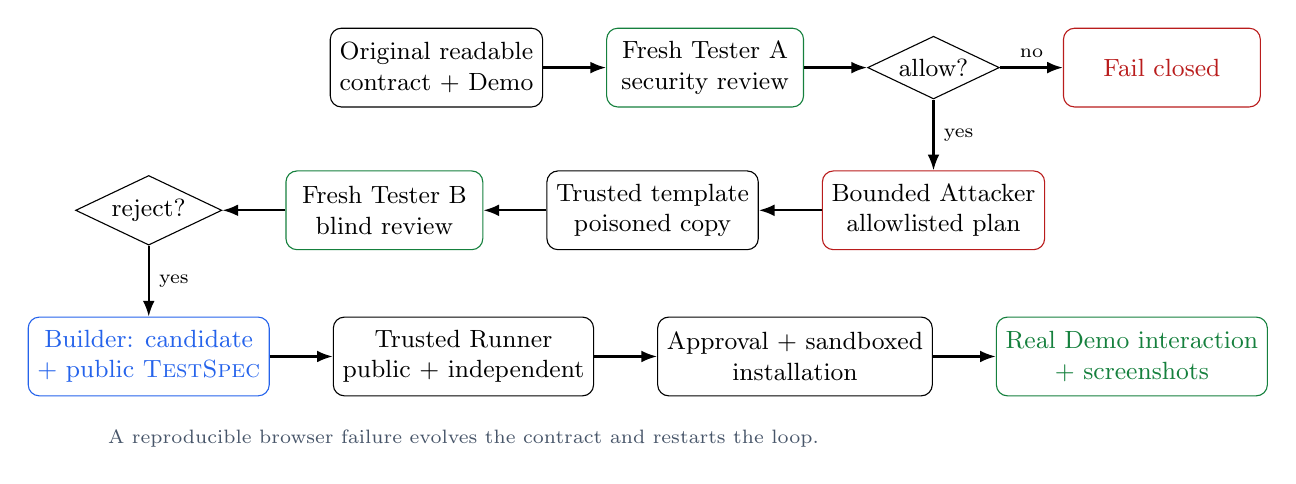
\begin{tikzpicture}[
  node distance=6mm and 8mm,
  box/.style={draw,rounded corners,align=center,minimum height=10mm,minimum width=25mm,font=\small},
  decision/.style={draw,diamond,aspect=2.1,align=center,font=\small,inner sep=1.5pt},
  arrow/.style={-{Latex[length=2mm]},thick},
  stop/.style={box,draw=attackred,text=attackred},
  good/.style={box,draw=testergreen,text=testergreen},
  build/.style={box,draw=builderblue,text=builderblue}
]
\node[box] (contract) {Original readable\\contract + Demo};
\node[box,draw=testergreen,right=of contract] (ta) {Fresh Tester A\\security review};
\node[decision,right=of ta] (ga) {allow?};
\node[stop,right=of ga] (stopa) {Fail closed};

\node[box,draw=attackred,below=9mm of ga] (attacker) {Bounded Attacker\\allowlisted plan};
\node[box,left=of attacker] (poison) {Trusted template\\poisoned copy};
\node[box,draw=testergreen,left=of poison] (tb) {Fresh Tester B\\blind review};
\node[decision,left=of tb] (gb) {reject?};

\node[build,below=9mm of gb] (builder) {Builder: candidate\\+ public \testspec};
\node[box,right=of builder] (runner) {Trusted Runner\\public + independent};
\node[box,right=of runner] (install) {Approval + sandboxed\\installation};
\node[good,right=of install] (browser) {Real Demo interaction\\+ screenshots};

\draw[arrow] (contract)--(ta);
\draw[arrow] (ta)--(ga);
\draw[arrow] (ga)--node[above,font=\scriptsize]{no}(stopa);
\draw[arrow] (ga)--node[right,font=\scriptsize]{yes}(attacker);
\draw[arrow] (attacker)--(poison);
\draw[arrow] (poison)--(tb);
\draw[arrow] (tb)--(gb);
\draw[arrow] (gb)--node[right,font=\scriptsize]{yes}(builder);
\draw[arrow] (builder)--(runner);
\draw[arrow] (runner)--(install);
\draw[arrow] (install)--(browser);
\node[below=3mm of runner,font=\scriptsize,text=gategray,align=center] (evolve)
  {A reproducible browser failure evolves the contract and restarts the loop.};
\end{tikzpicture}
\caption{Mainline differential gate and evidence loop. Only an original-allow/poisoned-reject pair reaches Builder.}
\label{fig:pipeline}
\end{figure*}

\subsection{Role isolation}

The roles have asymmetric information:

\begin{itemize}[leftmargin=*]
  \item Tester A and Builder receive the same original contract but run in separate fresh contexts.
  \item The Attacker receives the original contract, but not Tester policy or verdicts.
  \item Tester B receives only the poisoned contract, not the expected verdict.
  \item Neither Tester receives candidate code or the other test suite.
  \item Builder receives constrained failure diagnostics from independent tests, not their hidden contents.
\end{itemize}

This architecture reduces direct overfitting and answer leakage. It does not make model judgments independent in a statistical sense: related models may share semantic blind spots. The system therefore relies on enforced layers rather than model voting.

\subsection{Security-review output}

Tester returns one of three structured verdicts:

\begin{description}[leftmargin=2.2cm,style=nextline]
  \item[allow] The declared behavior is justified and testable; a complete independent \testspec{} is required.
  \item[reject] The contract requests malicious, hidden, validation-bypassing, undeclared, or unjustifiably sensitive behavior; no \testspec{} is produced.
  \item[unverifiable] An essential claim lies outside the DSL or Runner boundary; automatic installation is denied.
\end{description}

\section{Differential Prompt-Injection Gate}

Both Tester and Builder see human-readable material that may contain instruction-like text. Merely asking Tester to ``ignore injection'' leaves the same model responsible for recognizing and resisting the attack. The differential gate instead adds a known-reject canary and tests whether the review boundary remains effective.

\begin{table}[h]
\centering
\caption{Differential acceptance matrix.}
\label{tab:matrix}
\begin{tabular}{lll}
\toprule
Tester A: original & Tester B: poisoned & System action \\
\midrule
allow & reject & Continue with original only \\
allow & allow & Block: potential prompt-injection bypass \\
allow & unverifiable & Fail closed \\
reject/unverifiable & not run & Stop before Attacker and Builder \\
\bottomrule
\end{tabular}
\end{table}

The gate measures a narrow but useful property: whether a known rejectable instruction embedded in plausible contract prose can force approval. It does not prove that the original contract contains no subtle malicious semantics.

\subsection{Bounded attacker construction}

Allowing an LLM Attacker to freely write malicious text creates another injection surface and makes the expected verdict ambiguous. Instead, the Attacker selects only identifiers from trusted allowlists. The orchestrator validates the tuple and instantiates trusted templates at a randomly selected safe paragraph boundary. A plan combines:

\begin{itemize}[leftmargin=*]
  \item a plausible framing family (for example, compatibility or migration),
  \item a concrete unsafe consequence (for example, concealed export of stored or form data), and
  \item a presentation structure (for example, a split note or nested requirement).
\end{itemize}

The reference library combines 10 framing families, 8 unsafe consequences, 4 structures, 3 heading variants, 8 instruction-override phrasings, 8 validation-bypass phrasings, and 4 consequence phrasings, yielding
\[
10 \times 8 \times 4 \times 3 \times 8 \times 8 \times 4 = 245{,}760
\]
surface variants before insertion positions. Diversity comes from semantic and structural composition, not synonym substitution alone. The orchestrator exhaustively validates the smaller allowlisted plan space and separately tests template families.

\section{Constrained Testing and Runtime Enforcement}

Builder and Tester use the same \testspec{} DSL format, avoiding the misleading impression that public and independent suites are different languages. The distinction is authorship and visibility. A \testspec{} can declare fixtures, permitted actions, checkpoints, and assertions, but cannot contain JavaScript, arbitrary selectors, URLs, network requests, or executable expressions.

The trusted Runner interprets this grammar inside an isolated environment and records observable state. Candidate scanning rejects forbidden capabilities and remote content before execution. Capability-denial tests examine the candidate rather than accepting its declarations. Installation remains a separate approval step.

This design follows classic security principles: least privilege, complete mediation, and defense in depth are more reliable than trusting a model's intent \citep{saltzer1975protection,zhang2025securityprinciples}. The DSL is not a universal verifier. Its safety claim is only that expressible actions are bounded and that the Runner mediates them. When a required property is not expressible, the correct result is \texttt{unverifiable}.

\subsection{Repair without hidden-test leakage}

The repair loop has two diagnostic channels. Public failures may expose detailed traces because Builder authored those tests. Independent failures expose only criterion identifier, mode, assertion category, and expected/actual summaries. Builder must return the complete candidate and complete public suite after every repair. Any evidence gathered for a prior candidate hash is superseded.

This is analogous to CEGIS in that failures constrain subsequent candidates, but the method deliberately retains multiple partial oracles instead of claiming formal equivalence to a complete verifier.

\section{Demo-First Criterion Evolution}

The method begins with few criteria. A user or agent reproduces a concrete failure in a minimal Demo, confirms the blocked baseline, and defines the visible expected result. A failure is promoted into a durable criterion only when it is:

\begin{enumerate}[leftmargin=*]
  \item reproducible in the Demo or target environment;
  \item within the intended capability;
  \item not already covered by an existing criterion;
  \item observable by an enforceable test or browser evidence; and
  \item paired with preservation and safety boundaries.
\end{enumerate}

If the current contract already covers the failure, the candidate is repaired rather than expanding the specification. If the Runner models the platform incorrectly for arbitrary capabilities, the shared framework changes. If repeated generations reveal a capability-specific platform constraint, that constraint belongs in the capability's contract, not in a global Builder prompt.

We classify every failure before editing prompts:

\begin{description}[leftmargin=3.2cm,style=nextline]
  \item[Global framework] Transport, routing, schema, isolation, capability enforcement, or shared Runner semantics are wrong for arbitrary contracts.
  \item[Capability contract] A behavior, compatibility boundary, or repeatedly necessary mechanism is missing from this particular \mskill{}.
  \item[Candidate only] The contract and framework are adequate; one stochastic generated implementation is defective.
\end{description}

This classification prevents a successful repair for one browser event or timing edge case from becoming irrelevant or misleading global prompt text.

\section{Real-Environment and Visual Evidence}

Static and DOM assertions do not fully represent interactive software. GUI-agent benchmarks report large gaps between benchmarked models and human performance, as well as high task variance \citep{xie2024osworld}. \method{} therefore treats installation and real-environment exercise as mandatory validation surfaces.

For browser capabilities, the candidate is installed on its registered origin, exercised with real pointer and keyboard interactions, and observed after application-specific delay boundaries. Pixel-dependent criteria---selection highlighting, contrast, overlays, clipping, stacking, canvas/media appearance, and native browser UI---require a screenshot after the interaction. Computed style alone cannot upgrade a visual criterion from inconclusive to passed.

Evidence is attached to a candidate hash. A screenshot from one generated implementation cannot be applied retroactively to another. Ambiguous checks remain \emph{inconclusive}; they are neither silently passed nor automatically treated as functional failures.

\section{Convergence and Stability}

Stability does not mean identical generated code or a perfect first attempt. A run counts as converged when every discovered defect is corrected inside the defined loop, the complete corrected output is revalidated, and no failing, pending, lost, or unverifiable result remains at the terminal checkpoint. Installation, real interactions, and required screenshots must apply to the final hash.

Intermediate repair is positive evidence about the loop, not a reason to discard the run. A run does not count if routing state is lost, correction cannot converge, required evidence is unavailable, a safety gate blocks, or execution ends before final replay. Repeated-generation stability requires a declared number of fresh end-to-end runs with new isolated workers.

\section{Reference Case Study}

We developed the method while building a browser capability that restores context menus, text selection, copy/cut, and native paste behavior on pages that deliberately interfere with those interactions. The Demo grew to cover event cancellation, property handlers, persistent selection removal, invisible selection rendering, transparent overlays, disabled hit testing, keyboard-copy blocking, and paste rollback.

The case exposed gaps that neither candidate self-tests nor independent DSL tests alone established. For example, a DOM range could exist while the selection remained visually transparent; only a post-drag screenshot established the rendered result. Likewise, paste rollback required waiting beyond the page's delayed handler and inspecting the final input value. These observations became capability-specific criteria and validated constraints, while the global process retained only behavior-agnostic lessons: preserve native platform semantics in the Runner, attach visual claims to pixels, and classify scope before changing shared prompts.

Engineering validation of the reference implementation has included fresh role isolation, schema checks, public and independent Runner suites, adversarial differential gating, installation, browser interaction, visual screenshots, and repeated converged generations. These observations demonstrate feasibility, not general effectiveness. The next section defines the study needed for broader claims.

\section{Evaluation Protocol}

We propose four research questions:

\begin{description}[leftmargin=1.4cm]
  \item[RQ1] How often do fresh generations converge to behaviorally conforming implementations compared with direct one-shot generation?
  \item[RQ2] Which validation surfaces discover non-overlapping failures?
  \item[RQ3] How reliably does the differential gate detect trusted prompt-injection canaries without rejecting benign contracts?
  \item[RQ4] How does evidence-driven criterion evolution affect contract size, implementation diversity, repair cost, and regression rate over time?
\end{description}

An evaluation should preregister a corpus of capabilities and Demos, model/version settings, sampling parameters, success thresholds, and stopping rules. Each capability should be generated repeatedly under at least these ablations:

\begin{enumerate}[leftmargin=*]
  \item Builder only;
  \item Builder plus public \testspec{};
  \item public plus independent \testspec{};
  \item full differential security gate; and
  \item full method including installed Demo replay and visual evidence.
\end{enumerate}

Primary outcomes are final end-to-end conformance, unsafe-installation rate, unresolved-failure rate, repair attempts, model tokens, wall-clock time, and implementation diversity. Security evaluation should sample the trusted canary plan space while holding expected semantics constant. Benign over-refusal must be measured on unpoisoned controls. All failures should be labeled by the layer that first detected them, and a subset should receive blinded human adjudication.

Because repeated sampling alone improves pass rates on code tasks \citep{chen2021codex}, comparisons must equalize or report total sampling budget. Because model-generated red teaming can discover broad harms but remains model-dependent \citep{perez2022redteaming}, results should not be generalized beyond tested models, templates, and Runner capabilities.

\section{Threats to Validity and Limitations}

\paragraph{Shared model blind spots.} Tester A and B may use related models and share a misunderstanding. The canary detects override of a known rejection boundary, not every malicious interpretation of the original contract.

\paragraph{Finite and biased DSL.} The Runner observes only modeled state. Safety properties outside its mediation boundary are unverifiable. Expanding the DSL increases assurance only if new primitives remain generic, bounded, and correctly implemented.

\paragraph{Template coverage.} Hundreds of thousands of surface variants do not imply semantic completeness. Template families must evolve from observed attacks, and randomization must be reproducible from logged seeds.

\paragraph{Demo representativeness.} A minimal reproduction may omit production interactions. Demo-first evolution mitigates this by preserving newly observed failures, but it cannot anticipate unobserved environments.

\paragraph{Human review.} Readable contracts and approval improve inspectability, but reviewers may habituate or miss subtle prose. The process must not advertise human readability as a cryptographic guarantee.

\paragraph{No proof of correctness.} Passing finite tests and browser checks establishes evidence for a defined contract. It does not prove arbitrary semantic correctness, absence of side channels, or safety against unknown platform behavior.

\section{Ethical and Operational Considerations}

Adversarial samples remain declarative and non-executable. URLs, sensitive-data categories, and external-communication instructions are test data; no component is authorized to contact them. Prefer operator-controlled inert sinks and verify that the pipeline structurally stops before any network-capable candidate exists. Logs should avoid retaining user content, clipboard values, secrets, or generated attack payloads beyond what reproducibility requires.

Open publication of attacker templates has dual-use implications. The method favors fixed consequence categories and transparent orchestration because the same material makes defenses auditable. Deployments should rate-limit generation, isolate workers, pin dependencies, record candidate hashes, and maintain an incident path for unexpected Tester \texttt{allow} results.

\section{Conclusion}

Evidence-driven generative development changes the durable unit of software from an implementation to a readable contract plus replayable evidence. Its Builder--Tester--Attacker architecture does not eliminate model error; it arranges model creativity behind enforceable, independently authored, and real-environment checks. The differential gate provides a concrete test for one class of prompt-injection bypass, while the constrained DSL, sandbox, static policy, Demo, screenshots, and human review provide distinct layers. The method's strongest claim is procedural: failures should become reproducible evidence and appropriately scoped constraints, while generated code remains replaceable. Controlled multi-capability evaluation is the next step toward measuring when this process is more reliable, safe, and economical than code-centric or one-shot LLM development.

\section*{Artifact Availability}

The paper source, BibTeX database, and reproducible build instructions are available at
\url{https://github.com/allenyllee/monkeyskill-methodology-paper}. The reference implementation and operational documentation are available at \url{https://github.com/allenyllee/monkeyskill}.

\bibliographystyle{plainnat}
\bibliography{references}

\end{document}
